\documentclass{MYZJUMCM}
\usepackage{fontspec}
\setControlNumber{1231231} %队伍号
\setContestType{MCM} % contest type, only MCM or ICM allowed
\setProblemLetter{A} % choose problem A,B,C,D,E or F


%字体
\setmainfont{Times New Roman}
\setBibFilename{McmTexExample} % set bib file, without dot and suffix
\setPaperTitle{My Title111111} % set your title


%这里写总结文字。
\setSummary{This place is for summary.

This is another paragraph. 
}


\begin{document}
\showSummarySheet
\showContents % 正常编写,目录显示
\section{Chapter1}
\subsection{Chapter1-1}
The basic .tex file structure is as the following and comment for each corespending line is listed.

\begin{lstlisting}[style=latexstyle]
\showReferences         % show references
\end{lstlisting}

\subsection{Chapter1-2} 
Usually, the process can be executed as following:

\begin{itemize}
\item item1
\item item2
\end{itemize}


% subsection subsection_name (end)
\section{Introduction to mathematical typeseting within Latex}

We choose mathematical typeseting from \cite{tobias}.



\section{Some complements}
We put the source code of the HZNUMCM latex class file and this file on the gitHub \url{https://github.com/hznu-maguochun/HZNUMCM}, so that one use it can understand it. Any one, who want to use or improve it, is welcome. This class file also gives an idea about how to make a formatted file.

\showReferences

%\includepdf[pages=57-86,offset=0cm 0.5cm]{lshort.pdf}
\end{document}
